%%%%%%%%%%%%%%%%%%%%%%%%%%%%%%%%%%%%%%%%
% Class options                        %
%%%%%%%%%%%%%%%%%%%%%%%%%%%%%%%%%%%%%%%%
% Orientation:                         %
% portrait (default), landscape        %
%                                      %
% Paper size:                          %
% a0paper (default), a1paper, a2paper, %
% a3paper, a4paper, a5paper, a6paper   %
%                                      %
% Language:                            %
% english (default), norsk             %
%%%%%%%%%%%%%%%%%%%%%%%%%%%%%%%%%%%%%%%%
\documentclass[landscape]{uioposter}


\usepackage{lipsum}                                % Dummy text
\usepackage[figwidth = 0.98\linewidth]{todonotes}  % Dummy image (and more!)
\usepackage[absolute, overlay]{textpos}            % Figure placement
\setlength{\TPHorizModule}{\paperwidth}
\setlength{\TPVertModule}{\paperheight}
\usepackage{subcaption}
\usepackage{graphicx}


\title{TART Interferometer Imaging Pipeline}
\author
{%
    Jason Jackson%\inst{1}
    \and
    Supervisor: Dr. TL Grobler%\inst{2}
}
% Optional:
\institute
{
    \inst{} Stellenbosch University \and Department of Computer Science
}
%% Or:
%\institute{Contact information}


% % Remove footline:
% \setbeamertemplate{footline}{}


\begin{document}
\begin{frame}
\vspace{-0.8cm}
\begin{columns}[onlytextwidth]


\begin{column}{\textwidth/3 - 2cm}
    \begin{block}{Introduction}
        The field of radio interferometry entails the astronomical observation of radio celestial emission using special equipment called radio interferometers. Radio interferometers are arrays of radio antennas that work together to capture celestial radio emissions.\\
        In this project we create an imaging pipeline for a specific radio interferometer named TART, which was created in Otago University New Zealand. This pipeline creates images for the TART interferometer in Stellenbosch and New Zealand.
    \end{block}

    \begin{block}{How the pipeline works}
        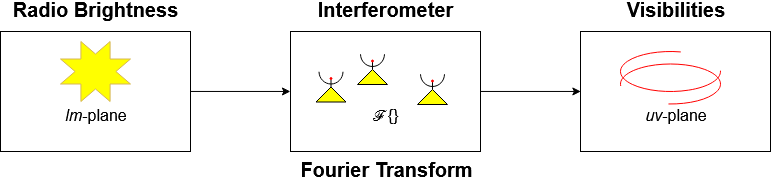
\includegraphics[scale=1.2]{Images/Radio_Interferometry.png}
        If one were to take the sky brightness distribution, and apply a Fourier transform to it, this would create something called visibilities. These visibilities are what an interferometer samples, the Fourier transform of the sky brightness distribution. If an inverse Fourier transform is applied to these visibilities then an image of the sky brightness should be obtained, due to the nature of Fourier transformation.
    \end{block}
\end{column}


\begin{column}{\textwidth/3 - 2cm}
    \begin{block}{Results}
        \vspace{-3cm}
        \begin{figure}
            \begin{subfigure}[b]{0.49\textwidth}
                \includegraphics[scale=0.7]{Images/7-11-19_13:41_SA_PIPE_CIRCLES.png}
                \caption{Pipeline Image}
                \label{fig:Pipe}
            \end{subfigure}
            \begin{subfigure}[b]{0.49\textwidth}
                \hspace{2cm}
                \includegraphics[scale=0.9]{Images/7-11-19_13:41_SA_WEB_CIRCLES.png}
                \vspace{1.5cm}
                \caption{API Image}
                \label{fig:API}
            \end{subfigure}
            \caption{Pipeline and web API image comparisons}
            \label{fig:Comparison}
        \end{figure}
        \vspace{-1cm}
        Figure \ref{fig:Pipe} and Figure \ref{fig:API} are observations that were taken at the same time
        through the pipeline and the web API for TART; there are points circled on the images that are common to both of them.
    \end{block}

    \begin{block}{Conclusion}
        The pipeline is able to produce images of the sky that match what the web API is able to produce.
        The pipeline produces good images, however, there is a lot of noise around the point sources. This is due to the fact that TART cannot sample the entire \textit{uv}-plane.
    \end{block}
\end{column}


\begin{column}{\textwidth/3 - 2cm}
    % \begin{block}{Technology Stack}
    %     
\includegraphics[scale=1.6]{Images/f9b9eec6-4123-4c1f-a993-a82cdae706fc.png}
    %     
\includegraphics[scale=0.3]{Images/768px-Python-logo-notext.png}
    % \end{block}
    
    \begin{block}{TART}
        \vspace{-1cm}
        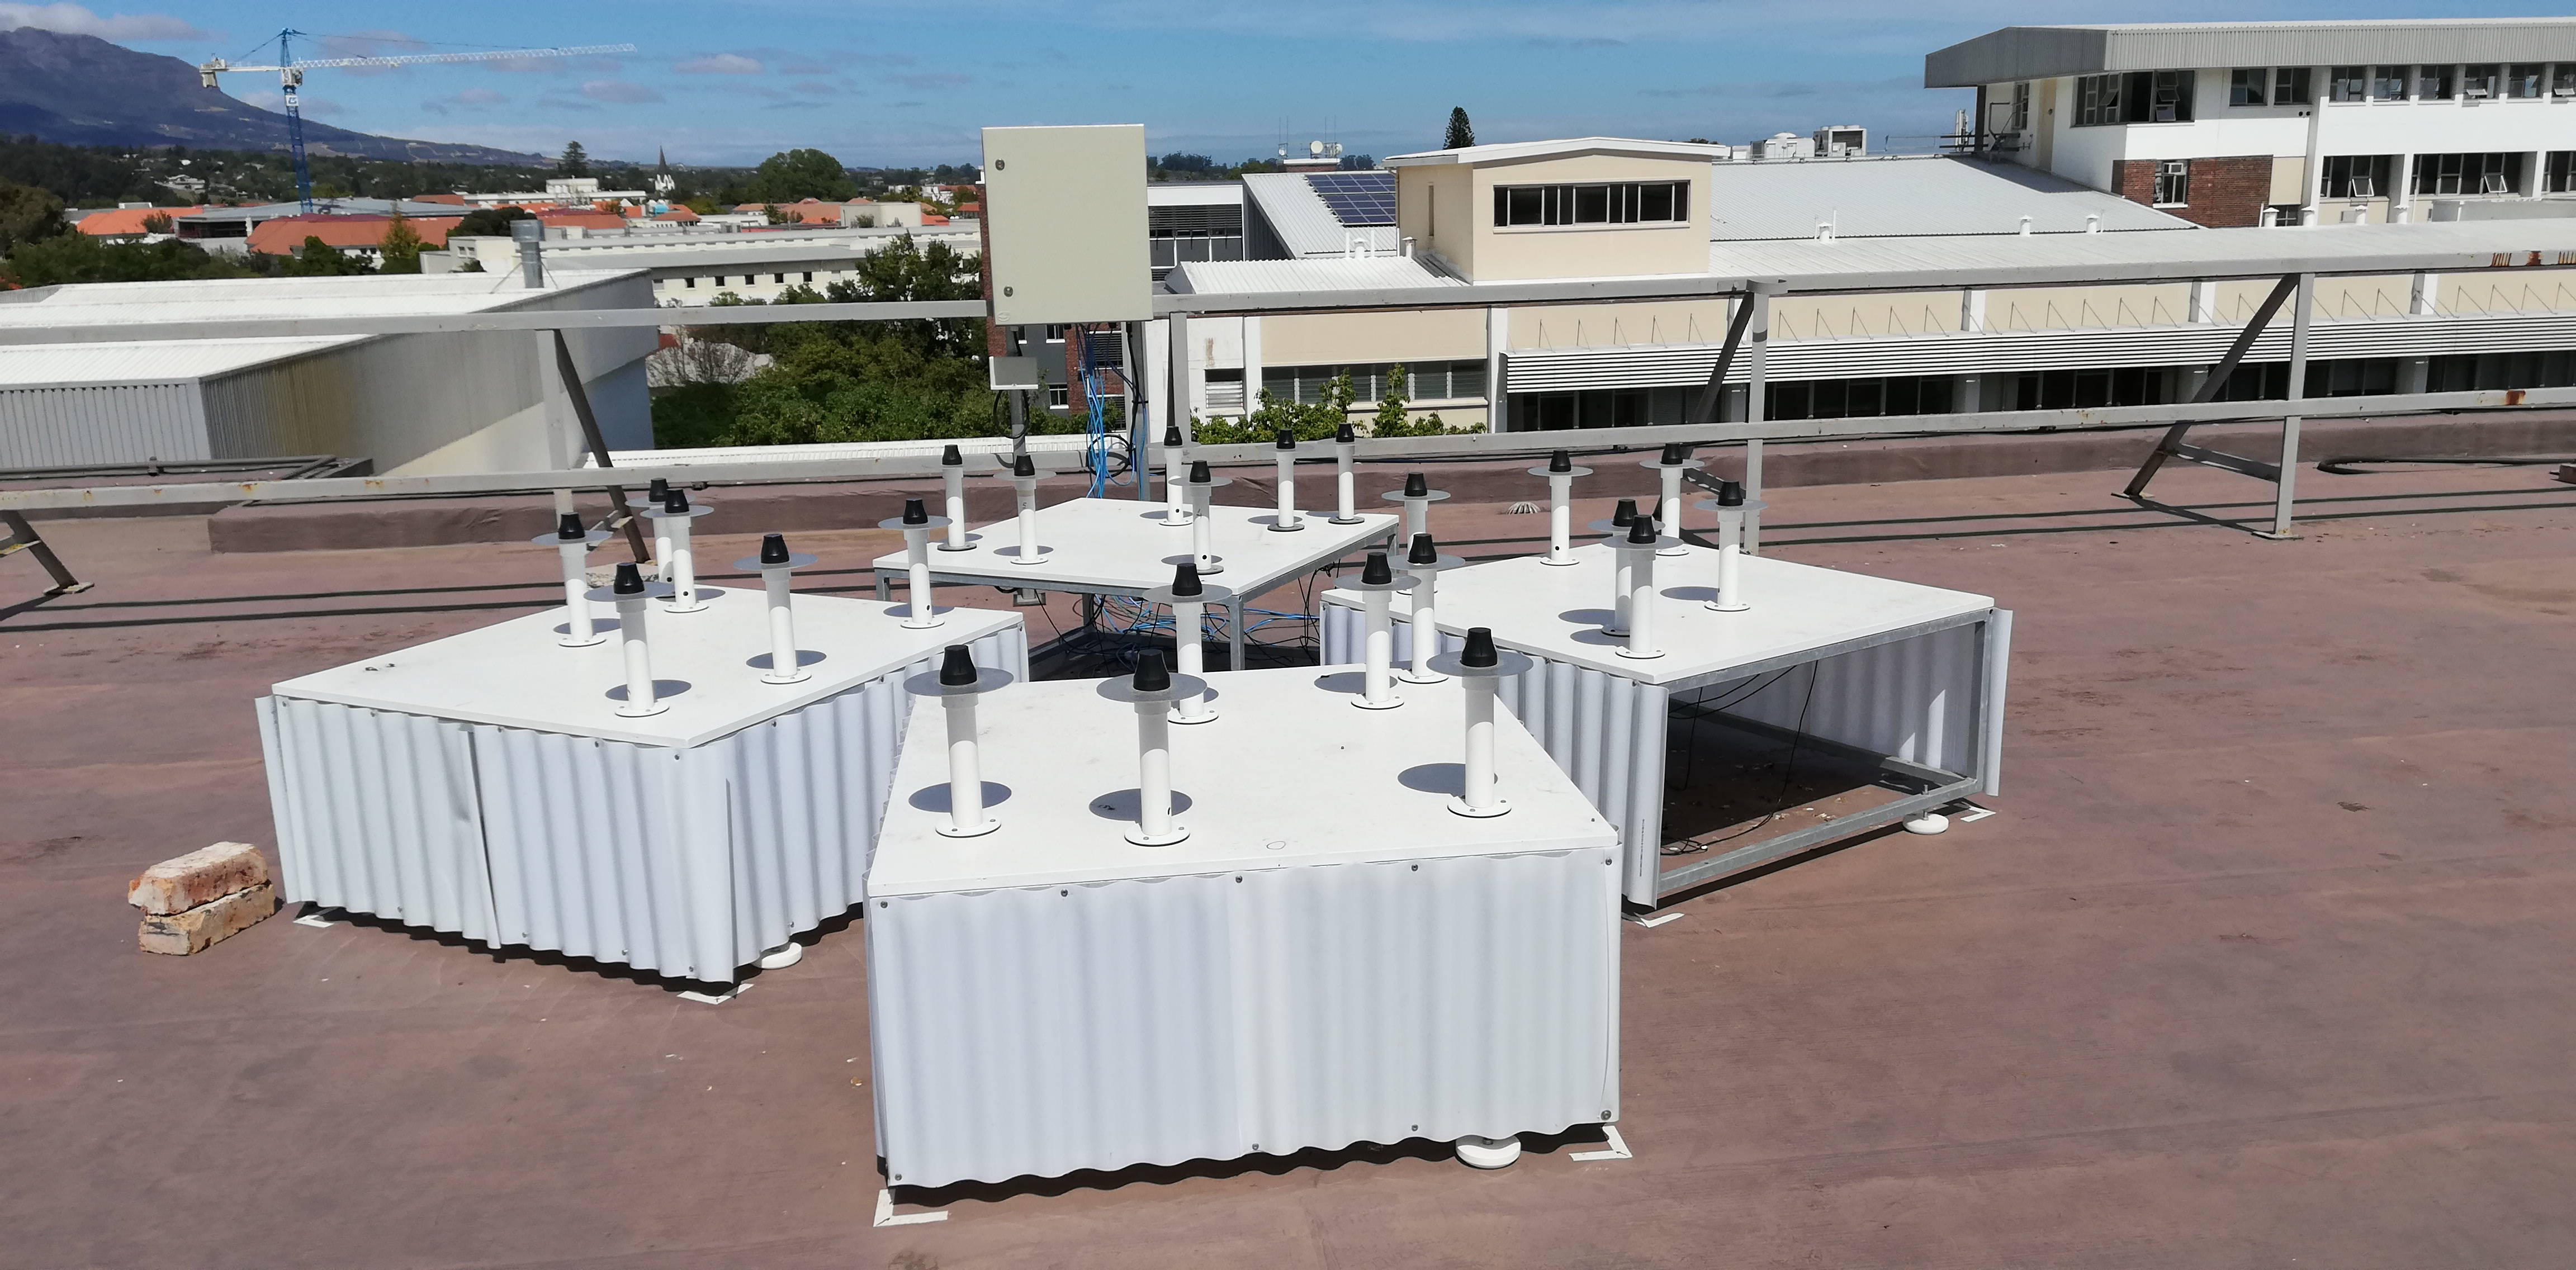
\includegraphics[scale=0.2]{Images/IMG_20190320_121412.jpg}
        Stellenbosch University has a TART interferometer deployed on top of the Electrical Engineering building; this is the interferometer that was used in the pipeline to obtain all the results. TART is a whole sky interferometer, meaning the images that are produced from it sample the whole sky, which leads to the images having a lot of noise in them as there is no focus on a specific area of the sky.
    \end{block}
    \vspace{-0.8cm}
    \begin{block}{Acknowledgements}
        Thank you to Dr. DJ Ludick for allowing the use of the Electrical Engineering TART interferometer and for explaining how to work with it.
    \end{block}


\end{column}

\vspace{2cm}

\end{columns}
\begin{columns}
    \begin{column}{\textwidth}
        \begin{block}{Future Work}
            The pipeline works as intended, it is able to generate images from the TART visibilities, however, these images are not very clear. This can be improved by adding extra steps to the pipeline. If a calibration step is applied to the pipeline, then the images that are produced will not contain as many errors due to false readings. \\
            If a deconvolution step is applied then the point sources in the images will not contain as much noise around them, leading to a cleaner image with more easily identifiable point sources.\\
            If both of these steps are added to the pipeline then the images that are produced will be far more clear which will make the pipeline even better.
        \end{block}
    \end{column}
\end{columns}

\begin{textblock}{0.5}(0.12, 0.92)
    \color{white}
    \sffamily
    % \textbf{Write here using textblock}
    % \\
    % Such as contact information or references
\end{textblock}


\end{frame}
\end{document}